\documentclass[a4paper]{article}

\usepackage{color}
\usepackage{url}
\usepackage[T2A]{fontenc} 
\usepackage[utf8]{inputenc} 
\usepackage{graphicx}

\usepackage[english,serbian]{babel}


\usepackage[unicode]{hyperref}
\hypersetup{colorlinks,citecolor=green,filecolor=green,linkcolor=blue,urlcolor=blue}

\newtheorem{primer}{Primer}[section]

\begin{document}

\title{Poređenje različitih vrsta prenosa podataka na mobilnom telefonu\\ \small{Seminarski rad u okviru kursa\\Tehničko i naučno pisanje\\ Matematički fakultet}}

\author{Andrija Soković\\ 
\small{andrijasokovic@gmail.com}
\and
Nenad Pešić\\
\small{pesicnenad28@gmail.com}
\and
Vojin Knežević\\
\small{knezevic.vojin@gmail.com}
\and 
Vukašin Cupara\\
\small{vukasin.cupara2003@gmail.com} 
}
\date{14.~novembar 2022.}
\maketitle

\abstract{
Ovaj tekst obuhvata vrste prenosa podataka na mobilnom telefonu. Upoznaćemo se sa različitim tipovima prenosa, naučićemo kako one funkcionišu i gde ih možemo sresti. Moramo spomenuti da iako na prvo pogled nam tematika ne zvuči komplikovano, ona je zaista kompleksna i nije ni malo jednostavna.

\tableofcontents

\newpage

\section{Uopšteno o prenosu podataka u računarstvu}
\label{sec:uvod}
\textbf{Razmena podataka} predstavlja proces pouzdanog slanja podataka izmedju dva ili većeg broja učesnika u komuniciranju. Ovim procesom moguće je slati mnogobrojne vrste podataka od kojih su najčešći: računarski fajlovi, digitalizovani signali slike, telemetrijski merni rezultati (npr. Podaci o merenjima temperature sa nekog senzora), centralne baze za nadgledanje itd.
U osnovnom obliku razmene podataka moguće je ostvariti komunikaciju između dva direktno povezana računara putem odgovarajućeg medijuma za prenos. Međutim, vrlo često, ovakav vid komunikacije nije dovoljan i pojavljuje se potreba za povezivanjem više računara. Tada je najpovoljnije povezati uređaj u neku već postojeću mrežu koja je organizovana po određenim standardima. \\
Iako ne postoji opšta (zvanična) kategorizacija računarskih mreža, neformalno, mi računarske mreže možemo podeliti u dve grupe:
\begin{itemize}
\item Broadcast mreže (emisija svima)
\item Point-to-point (između 2 računara)
\end{itemize} 
Pored ove logičke podele računare fizički možemo povezivati različitim medijumima za prenos. Tu takođe možemo ostvariti neformalnu podelu na dve kategorije mreža u zavisnosti od vrste medijuma koji se koristi pri razmeni podataka:
\begin{itemize}
\item Žične računarske mreže (fizički medijum, npr. Bakarni kabl)
\item Bežične računarske mreže (medijum je etar, vazduh))
\end{itemize} 

\section{Bežične mreže}
Mobilni telefoni dizajnirani su na način koji predviđa upotrebu baš bežičnih mreža za međusobnu komunikaciju. Bežične mreže, prema svojoj topologiji možemo razvrstati u tri zasebne kategorije:
\begin{itemize}
\item Ad-hoc
\item Celularne (ćelijske)
\item Point-to-point
\end{itemize} 
    \subsection{Ad-Hoc}
Uspostavljanje komunikacije među uređajima vrši se direktno, bez unapred obezbeđene infrastrukture. Omogućava se veza „svako sa svakim“ bez pristupnih stanica. Poruka propagira kroz mrežu koristeći čvorove kroz koje prolazi, svaki uređaj u mreži postaje i čvor. Pod terminom čvor, podrazumeva se svako mesto u mreži na kojem može doći do „grananja“, odnosno, promene smera paketa (poruke) koja se prosleđuje kroz mrežu. Ovakve mreže su pogodne za komunikaciju između manjih grupa korisnika na malom rastojanju i primenjuju se uglavnom tamo ge je neophodno brzo uspostaviti privremenu mrežu.\\
Na slici \ref{fig:adhoc} prikazan je dijagram Ad-Hoc mreže.
\newpage

\begin{figure}[h!]
\begin{center}
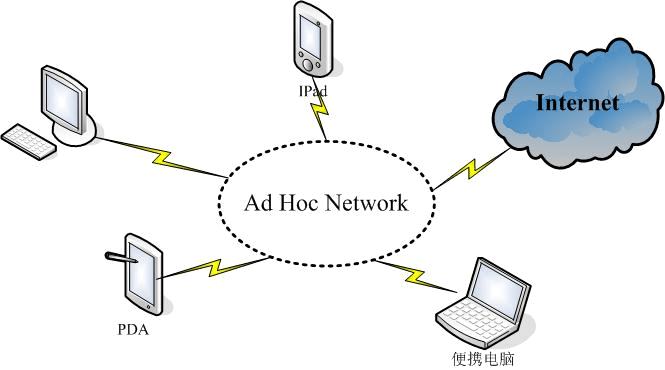
\includegraphics[scale=0.35]{AdHoc.png}
\end{center}
\caption{Ad-Hoc \cite{AdHoc}}
\label{fig:adhoc}
\end{figure}



    \subsection{Ćelijske mreže}
 Kod mreža sa ćelijskom topologijom uređaji ne mogu da komuniciraju direktno između sebe, već je neophodno da se sva komunikacija vrši preko unapred postavljenih pristupnih stanica. U ovakvim mrežama za komuniciranje je neophodno da postoji određena infrastruktura. Izras ćelijske mreže odnosi se na to da se jedno celo geografsko područje deli na određeni broj manjih područja pokrivenosti pristupnih stanica, odnosno ćelija.

    \subsection{Point-to-point}
\textbf{Point to point} mreže omogućavaju komunikaciju tačno dva uređaja bez potrebe za dodatnom infrastrukturom. Ovakve mreže koriste se uglavnom za privremenu komunikaciju dva uređaja koja se međusobno nalaze na maloj udaljenosti.

\section{Bezbednost}	
\label{sec:Bezbednost}

Kao važna karakteristika svake računarske mreže ubraja se I bezbednost iste. Različite vrste mreža podlozne su različitim napadima I obezbeđene su različitim metodama zaštite.
Uopšteno posmatrajući postoje tri različite vrste napada na mrežu (bežičnu mrežu):

\begin{itemize}
    \item Napadnuta fizička sigurnost mreže
    \item Neautorizovani napadi i prisluškivanje
    \item Ugrožavanje bezbednosti unutar same mreže od strane autorizovanog korisnika
\end{itemize}


\section{Vrste bežičnih mreža koje koriste mobilni telefoni}
\label{vrste_mreza_na_telefonu}

Nakon uspostavljanja osnovnih podela I karakteristika bežičnih mreža uopšteno, treba posmatrati I različite standarde, odnosno različite tehnologije bežične komunikacije koje koriste mobilni telefoni. Ipak pre pominjanja samih tehnologija, neophodno je izvršiti još jednu kategorizaciju istih prema nameni I području koje iste pokrivaju:

\begin{itemize}
    \item WWAN (Wireless Wide Area Network)
    \item WLAN (Wireless Local Area Network)
    \item WPAN (Wireless Personal Area Network)
\end{itemize}
    \subsection{WWAN (Wireless Wide Area Network)}
WWAN je mreža koja pokriva veliko geografsko područje. Ona vrši komunikaciju rastavljanjem “poruke” (podatka koji želimo da pošaljemo) na veliki broj malih delova koji se nazivaju paketi. U WWAN spadaju mrežne tehnologije poput: \textbf{LTE}, \textbf{GSM}, \textbf{CDPD}. 
        \subsubsection{GSM}
GSM tehnologija je prva verzija razmene podataka koja se (u svojoj novijoj realizaciji) I dalje koristi pri povezivanju telefona na mobilnu mrežu. Ovo je druga generacija mobilnih mreža (tzv. 2G). Razvijena je početkom devedesetih godina prošlog veka.
GSM koristi ćelijsku topologiju mreže. Upotrebljava se više baznih stanica koje pokrivaju svoja geografska područja (do 35 kilometara dometa). Ovo je prva verzija mobilne mreže koja koristi digitalnu tehnologiju za komunikaciju.
Svaka bazna stanica ima frekvenciju na kojoj radi I oblast koju pokriva (ćeliju). Ćelije se šematski prikazuju kao pravilni šestougaonici, čime se omogućava da su sve susedne stanice na istoj udaljenosti. Pri ovoj podeli, svake dve susedne stanice moraju da koriste različite frekvencije kako ne bi smetale jedna drugoj. \\
Glavne usluge koje GSM pruža su:
\begin{itemize}
    \item Prenos govora
    \item Prenos podataka (9.6 Kb/s)
    \item Slanje SMS (Short Message Service) poruka
\end{itemize}
Mobilni uređaj, koji pristupa mreži,  sastoji se od samog mobilnog telefona (terminala) i memorijske kartice, takozvane SIM (Subscriber Identity Module) kartice
\begin{itemize}
    \item Mobilni uređaj se jednoznačno identifikuje IMEI brojem (International Mobile
Equipment Identity) tj. međunarodnim brojem za identifikaciju mobilnog uređaja.
    \item SIM kartica sadrži međunarodni broj za identifikaciju pretplatnika IMSI
(International Mobile Subscriber Identity) kojim se pretplatnik najavljuje na sistem,
zatim, tajni kod za verifikaciju i druge informacije.
    \item IMEI i IMSI brojevi su nezavisni. SIM kartica može da se zaštiti od neovlašćenog
korišćenja lozinkom ili ličnim identifikacionim brojem.
\end{itemize} 
Na slici \ref{fig:GSM} je prikazan uprošćen dijagram GSM mreže.
























\end{document}
